% TEMPLATE for Usenix papers, specifically to meet requirements of
%  USENIX '05
% originally a template for producing IEEE-format articles using LaTeX.
%   written by Matthew Ward, CS Department, Worcester Polytechnic Institute.
% adapted by David Beazley for his excellent SWIG paper in Proceedings,
%   Tcl 96
% turned into a smartass generic template by De Clarke, with thanks to
%   both the above pioneers
% use at your own risk.  Complaints to /dev/null.
% make it two column with no page numbering, default is 10 point

% Munged by Fred Douglis <douglis@research.att.com> 10/97 to separate
% the .sty file from the LaTeX source template, so that people can
% more easily include the .sty file into an existing document.  Also
% changed to more closely follow the style guidelines as represented
% by the Word sample file. 

% Note that since 2010, USENIX does not require endnotes. If you want
% foot of page notes, don't include the endnotes package in the 
% usepackage command, below.

% This version uses the latex2e styles, not the very ancient 2.09 stuff.

% Updated July 2018: Text block size changed from 6.5" to 7"

\documentclass[letterpaper,twocolumn,10pt]{article}
\usepackage{usenix2019,epsfig,endnotes}

\usepackage{pgfplots}
\pgfplotsset{compat=newest}


\begin{document}

%don't want date printed
\date{}

%make title bold and 14 pt font (Latex default is non-bold, 16 pt)
\title{\Large \bf 9Back : Making Our Plans Great Again}

%for single author (just remove % characters)
\author{
{\rm Maxwell Bland}
\and
{\rm Leon Cheung}\\ \\
University of California, San Diego
\and
{\rm Kilian Pfeiffer}\\
% copy the following lines to add more authors
% \and
% {\rm Name}\\
%Name Institution
} % end author

\maketitle

% Use the following at camera-ready time to suppress page numbers.
% Comment it out when you first submit the paper for review.
\thispagestyle{empty}


\subsection*{Abstract}
The following paper describes a set of benchmarks run on the Plan 9 operating system. In particular, it uses the only actively developed branch, 9FRONT "RUN FROM ZONE!" (2018.09.09.0 Release). The goal of this project is to provide researchers and enthusiasts with greater insight into the current state of the operating system's performance and capabilities of interaction with hardware. Through tests of CPU, Memory, Network, and File System operations, we will gain insight on bottlenecks in the system's performance and the interactions between low-level (hardware) and high-level (OS) system components. These performance statistics will be contrasted with subjective experiences of ``responsiveness''.

\section{Introduction}

Plan 9 from Bell labs is a distributed operating system which emerged around the 1980's. It built upon the ideas of UNIX, but adopted an ideology that ``everything is a file''. Although the system was marketed in the 90's, it did not catch on, as prior operating systems had already gained enough of a foothold. Eventually, during the 2000's, Bell Labs ceased development on Plan 9, meaning official development halted. Unofficial\footnote{This is debatable. If you adopt an orphan, are they not your official child?} development continues on the 9front fork of the codebase, with new support for Wi-Fi, Audio, and everything anyone could ever want or need. 

The experiments were performed as a group using a shared codebase and a single machine described in the following section. The measurements were performed via programs written in Plan 9's \textit{special} version of C 99 and Alef, both described in the original Plan 9 paper todo{cite}. The compilers used were the x86 versions of Plan 9's C compiler and Alef compiler, 8c and 8al respectively. The compilers were run with no special optimization settings. Version numbers are not available. Measurements were performed on a single machine running Plan 9 directly from hardware; given the nature of the Plan 9 system, additional metrics could be established for networked file systems and CPU servers; these measurements were not done for sake of simplicity, and because results under these conditions should be inferrable from the results cataloged within this paper.

\section{Machine Description}

We ran this beautiful operating system of the gods on a Thinkpad T420, the machine of true developers.

{\tt \small
\begin{verbatim}
    Processor: model, cycle time, cache sizes (L1, L2,
      instruction, data, etc.)
      Intel(R) Core(TM) i5-2520M CPU @ 2.50GHz (Sandy Bridge)
      cache size 3072 KB
      L1$	128 KiB	
        L1I$	64 KiB	2x32 KiB	8-way set associative	 
        L1D$	64 KiB	2x32 KiB	8-way set associative	write-back
      L2$	512 KiB 2x256 KiB	8-way set associative	write-back
      L3$	3 MiB   2x1.5 MiB	12-way set associative	write-back
      cpu family 6
      model 42
      stepping 7
      siblings 4
      cores 2
      fpu yes
      fpu_exception yes
      fpu_exception yes
      bogomips 4986.98
      clflush size 64
      cache_alignment 64
    Details at https://en.wikichip.org/wiki/
    intel/core_i5/i5-520m 

    Memory bus
      DDR3-1333
      i/o-bus-frequency: 666MHz
      bus-bandwith:  10656 MB/s
      memory-clock:  166MHz
      Column Access Strobe (CAS) latency:

    I/O bus
      SataIII-speed: 600MB/s

    RAM size
      8 GB
    Disk: capacity, RPM, controller cache size
      Samsung SSD 860 EVO 500GB
      Capacity: 500GiB
      RPM: 550MB/s read, 520 MB/s write
       and 98,000 IOPS (Read QD32)
      Controller Cache Size: 512MB 
    Network card speed:
     Intel 82579 LM Gigabyte: 1Gb/s
     intel Centrino Ultimate-N 6300: 450 Mbps
      
    Operating system (including version/release) 
      9FRONT "RUN FROM ZONE!" (2018.09.09.0 Release)
\end{verbatim}
}

\section{Experiments}

For each section, we report the base hardware performance, make a guess as to how much overhead software will add to base hardware performance, combine these two into an overall prediction of performance, and then implment and perform the measurement. In all cases, we run the experiment multiple times, and calculate the standard deviation across measurements. We use the \texttt{cycles()} syscall to record the timestamp. Dynamic CPU frequency scaling was disabled for all trials, and all trials were restricted to a single core.

\subsection{Measurement Overhead (Reading Time)}

The following section reports overheads of reading time. One trial involves looping over 16 \texttt{cycles} timing calls, $2^{16}$ times. We average out for each call of \texttt{cycles}, and we do 64 trials altogether.

Since we imagine getting the current cycles clock is a fast operation, so we
estimate the hardware performance to be on the scale of nanoseconds, since one
clock cycle takes approximately 1 nanoseconds. We think that the
\texttt{cycles} call should do something similar to reading from the cycle
counter, so it may be a bit slower, perhaps on the order of 10ns.
[https://www.7-cpu.com/cpu/SandyBridge.html]

The software cost of this, however, will be tremendous, since that value must
be moved out from a register and potentially to a variable, and a syscall must
be made, the result might be aroudn 10 to 30 times the hardware cost.

This would put our predicted cost at around 100 to 300 nanoseconds.

\subsection{Measurement Overhead (Loop Overhead)}

In order to measure the loop overhead, we took the time at the end of a loop
iteration and at the start of a loop iteration, and find the difference between
those to measure the loop overhead time. We repreat this 16384 times within
each trial, and perform 64 trials. We average over all of these trials.

The cost of doing a single for loop based branch in hardware is also very low.
Assuming a compare, jump, and register increment takes 3 cycles, and adding
2 cycles for rare branch mispredictions, the loop overhead should be around
5 cycles. Adding software uncertainties, the loop overhead could be about
50 nanoseconds.
[https://www.7-cpu.com/cpu/SandyBridge.html]

Software, again, will slow this down, as well as the rest of the operating
system. Other system processes may need the processor, data may not be in the
carch, and thus the latency might be 20 times this, the same as a reference to
the L2 cache, roughly.

Thus, our predicted cost is around 2 microseconds.

\begin{figure}
	\centering
    \begin{tabular}{lll}
      & Reading (ns) & Loop (ns) \\
Hardware Guess  & 100 & 2\\
Software Multiplier & 10-30 & 10 \\
Prediction & 1-3 usec & 20\\
Average  & 11 & 17.2 \\
Std Dev. & 0 & 0
\end{tabular}
\caption{Measurement Overheads}
\label{tab:generaloverheads}
\end{figure}


\subsection{Procedure Call Overhead}

In measuring the function overhead, we created functions of zero to seven integer arguments,
we then proceeded to call eacah of these functions 20000
times, and found the average time taken over these 20000 calls. Overall, increment overhead was almost non-existent.

The hardware cost of a procedure call using the standard c calling convention should not be that high, as it is almost all done in registers. The caller pushes the arguments to the stack (very little cost), saves the return address, the frame pointer, and calls the function. The hardware cost of this should be more than a for loop, but still reasonable, maybe roughly equitable since there are no comparisons or complex operations. Thus, somewhere on the range of 150ns to 200ns would seem reasonable, maybe even 100ns.
[https://www.7-cpu.com/cpu/SandyBridge.html]

The software cost of this is is probably about the same as the measurement overhead and for loop overhead, since we still may need to context switch to another process, as well as handle interrupts, etc. So I would reason that it would be around 20x the hardware cost.

This puts our prediction for the cost to be somewhere between 2000 nsec and 4000 nsec. Arguments shouldn't really effect the speed of a function call under our system.

\begin{figure}
	\centering
\begin{tabular}{lll}
Hardware Guess       & 150 nsec & \\
Software Multiplier Guess       & 20x &  \\
Prediction       & 3000 usec &  \\
Num Args & Average    & Std Dev.   \\
0        & 2.110 usec & 0.191 usec \\
1        & 2.104 usec & 1.248 usec \\
2        & 2.118 usec & 0.346 usec \\
3        & 2.113 usec & 0.571 usec \\
4        & 2.108 usec & 0.213 usec \\
5        & 2.120 usec & 0.915 usec \\
6        & 2.111 usec & 2.165 usec \\
7        & 2.108 usec & 0.321 usec
\end{tabular}
\caption{Procedure Call Overheads}
\label{tab:proccalloverheads}
\end{figure}

\subsection{System Call Overhead}

To measure the syscall overhead, we used the \texttt{errstr(2)} syscall, in
particular, \texttt{rerrstr(char*, vlong)}. \texttt{reerrstr} reads the error
string for the error of a previous syscall, and does not clear the errstr
buffer. Within each trial, we performed the syscall 16384 times, and averaged
over 64 trials.

Data from IBM puts the cost of making a system call on the Pentium processor in 1997/1995
to be 223 cycles, or roughly 1.68 usec for that processor. Our processor is much faster,
putting the timing at around 100 nsec.
%[https://www.ibm.com/developerworks/ community/blogs/kevgrig/entry /approximate_overhead_of_system_ calls9?lang=en]

It is likely that the overhead of a syscall beyond this is pretty high due to the
actual operations and implementation of the syscall operation. Thus, the cost could be 30 to
40x the hardware cost.

That puts our estimate at around 3 to 4 usec.

\begin{figure}
	\centering
    \begin{tabular}{ll}
            & System Call Overhead \\
    Hardware Guess  & 100 nsec  \\
    Software Multiplier  & 30-40x           \\
    Prediction  & 3-4 usec           \\
    Average  & 4.835 usec           \\
    Std Dev. & 0.056 usec          
    \end{tabular}
\caption{Syscall Overhead}
\label{tab:syscalloverheads}
\end{figure}

\subsection{Task Creation Time}

We measured process creation overhead in two different ways, one in which we
\texttt{rfork}'ed a new process without copying the parent state to the child,
and, \texttt{fork}, where the child will copy all of the parent's file
descriptors, and share the other state as normal. We do these 20000 times for
each type of \texttt{fork} and we average over all of these calls. This methodology
results from the fact that Plan 9 does not have kernel threads.

The hardware costs of a light fork should be much less than a heavy fork, since
resources do not need to be shared, but because our processes are minimal, it is
likely this difference is negligible. Still, this whole process will take tens of thousands to
millions of cycles, meaning thousands of microseconds, maybe 500 usec with a 1,000,000 cycles.
[http://ithare.com/infographics-operation-costs-in-cpu-clock-cycles/]

The software costs are most likely pretty low since Plan 9's rfork mechanism is relatively light
weight and similar to the Unix version of fork. It might only scale this already tremendous
runtime by a factor of two or so.

That puts our estimate at around 1000 usec for both fork operations.

\begin{figure}
	\centering
\begin{tabular}{lll}
        & Light Fork & Heavy Fork \\
Hardware Guess & 500 usec                 & 500 usec                  \\
Software Multiplier & 2x                 & 2x                  \\
Prediction & 1000 usec                 & 1000 usec                  \\
Average & 1080 usec                 & 1114 usec                  \\
Std Dev & 278 usec                  & 344 usec                  
\end{tabular}
\caption{Fork Overheads}
\label{tab:forkoverheads}
\end{figure}

\subsection{Context Switch Time}

Finally, to measure context switching, we created a pipe in a parent process,
and forked off a new child process. We forced a context switch by writing to
the pipe in the parent and then waiting for the child to read from the pipe
and terminate. We take the time between when the parent goes to sleep and when
the parent wakes up again after the child's termination. Then, we subtract
the overhead of reading from the pipe and closing the pipe (which happens in
the child), and divide the time in half to account for the two context switches.
We repeat this measurement 1000 times and use a new pipe each time. To take
the time of a context switch, we take the minimum time over all of these trials.

We estimated the base hardware cost of context switching while pinned to a single CPU to
be on the order of around 1100 ns based upon benchmarks done on the Intel E5-2620, another
Sandy Bridge processor model. [https://blog.tsunanet.net/2010/11/how-long-does-it-take-to-make-context.html]

The software cost to a context switch for Plan 9 is going to be huge. Probably on the order of 40x or something along these lines, since the OS needs to deal with scheduling and piping and I/O and virtual memory, etc..

This puts our prediction right around 44 usec.

\subsection{RAM Access Time}
To measure ram access time allocated a $1.6$ GB array on the heap, and iterated through it with changing stride size to hit L1, L2 cache and finally memory. The stride size gets increased by factor 1.1 for each iteration.

\begin{figure}
	\centering
	% This file was created by matplotlib2tikz vx.y.z.
	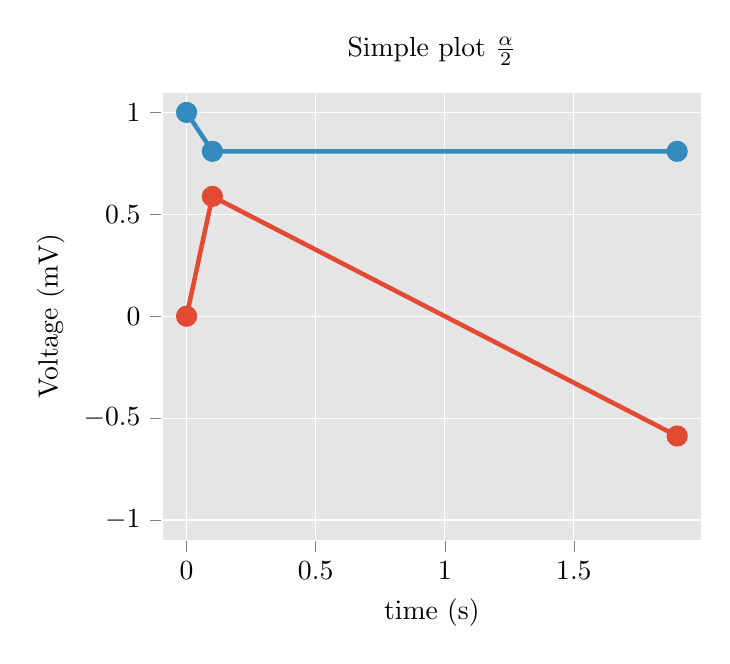
\begin{tikzpicture}
	
	\definecolor{color1}{rgb}{0.203921568627451,0.541176470588235,0.741176470588235}
	\definecolor{color0}{rgb}{0.886274509803922,0.290196078431373,0.2}
	
	\begin{axis}[
	title={Simple plot $\frac{\alpha}{2}$},
	xlabel={time (s)},
	ylabel={Voltage (mV)},
	xmin=-0.095, xmax=1.995,
	ymin=-1.1, ymax=1.1,
	tick align=outside,
	tick pos=left,
	xmajorgrids,
	x grid style={white},
	ymajorgrids,
	y grid style={white},
	axis line style={white},
	axis background/.style={fill=white!89.803921568627459!black}
	]
	\addplot [line width=1.64pt, color0, mark=*, mark size=3, mark options={solid}]
	table {%
		0 0
		0.1 0.587785252292473
		% [...]
		1.9 -0.587785252292473
	};
	\addplot [line width=1.64pt, color1, mark=*, mark size=3, mark options={solid}]
	table {%
		0 1
		0.1 0.809016994374947
		% [...]
		1.9 0.809016994374947
	};
	\end{axis}
	
	\end{tikzpicture}
	\caption{Ram access time with size of the memory region accessed on $x$ axis and latency in seconds on the $y$ axis}
\end{figure}

\begin{figure}
	\centering
\begin{tabular}{ll}
Hardware Cost  & 1100 nsec  \\
Software Multiplier  & 40x   \\
Prediction  & 44 usec    \\
Average  & 42.048 usec    \\
Std Dev. & 9.569 usec     \\
Min      & 12.491 usec   
\end{tabular}
\caption{Context Switch Overheads}
\label{tab:conswitchoverheads}
\end{figure}

\subsection{RAM Bandwidth}
We measured RAM bandwidth by allocating an array of $5 \cdot 10^6$ 4-byte
integers, and iterated through it to measure read and write bandwidth. For the
write bandwidth, we use \texttt{memset} to write to the entire array. In order
to measure the read bandwidth, we looped through the entire array, referencing
each integer element one by one, and compensated for the loop overhead after
averaging over all the times.

\begin{figure}
	\centering
    \begin{tabular}{l r r}
      & Bandwidth (GiB/s)\\
      Theoretical Maximum r/w & 10\\
      Software Multiplier & 0.8 \\
      Prediction & 8\\
                   & Average & Std Dev.\\
      Write & 6.879842 & 1.9829 \\
      Read & 9.109494 & 1.2845
\end{tabular}
\caption{Memory Bandwidth}
\label{tab:memorybandwidth}
\end{figure}

\subsection{Discussion}
\textit{Compare the measured performance with the predicted performance. If they are wildly different, speculate on reasons why. What may be contributing to the overhead?}
    Our hardware estimates were very, very rough. It'd be worthwhile to go back and double check these and discuss with our classmates on the numbers we arrived at.

    
    \textit{Evaluate the success of your methodology. How accurate do you think your results are?}
    Our results agree with the Plan 9 paper, which is suprising given that our processor is a bit faster. It will be worth it to discuss with Geoff our results and what we might try looking into going forward. It was hard to ensure we were taking the best approach. We certainly measured roughly what we wanted to measure.

\textit{Answer any questions specifically mentioned with the operation.}
The issue here is that there are no kernel threads in Plan 9, so some of the CPU measurement questions did not apply

\section{Conclusion}

We should try to correct our idea of hardware cycle counts for typical instructions and discuss the manners in which we chose to benchmark in order to make sure they are the absolute best way to measure these values, or something close to it. 

{\normalsize \bibliographystyle{acm}
\bibliography{../common/bibliography}}


%\theendnotes

\end{document}







